\documentclass[]{article}
\usepackage{lmodern}
\usepackage{amssymb,amsmath}
\usepackage{ifxetex,ifluatex}
\usepackage{fixltx2e} % provides \textsubscript
\ifnum 0\ifxetex 1\fi\ifluatex 1\fi=0 % if pdftex
  \usepackage[T1]{fontenc}
  \usepackage[utf8]{inputenc}
\else % if luatex or xelatex
  \ifxetex
    \usepackage{mathspec}
  \else
    \usepackage{fontspec}
  \fi
  \defaultfontfeatures{Ligatures=TeX,Scale=MatchLowercase}
\fi
% use upquote if available, for straight quotes in verbatim environments
\IfFileExists{upquote.sty}{\usepackage{upquote}}{}
% use microtype if available
\IfFileExists{microtype.sty}{%
\usepackage{microtype}
\UseMicrotypeSet[protrusion]{basicmath} % disable protrusion for tt fonts
}{}
\usepackage[margin=1in]{geometry}
\usepackage{hyperref}
\hypersetup{unicode=true,
            pdftitle={Reporducible Research:Peer Assessment 1},
            pdfborder={0 0 0},
            breaklinks=true}
\urlstyle{same}  % don't use monospace font for urls
\usepackage{color}
\usepackage{fancyvrb}
\newcommand{\VerbBar}{|}
\newcommand{\VERB}{\Verb[commandchars=\\\{\}]}
\DefineVerbatimEnvironment{Highlighting}{Verbatim}{commandchars=\\\{\}}
% Add ',fontsize=\small' for more characters per line
\usepackage{framed}
\definecolor{shadecolor}{RGB}{248,248,248}
\newenvironment{Shaded}{\begin{snugshade}}{\end{snugshade}}
\newcommand{\KeywordTok}[1]{\textcolor[rgb]{0.13,0.29,0.53}{\textbf{#1}}}
\newcommand{\DataTypeTok}[1]{\textcolor[rgb]{0.13,0.29,0.53}{#1}}
\newcommand{\DecValTok}[1]{\textcolor[rgb]{0.00,0.00,0.81}{#1}}
\newcommand{\BaseNTok}[1]{\textcolor[rgb]{0.00,0.00,0.81}{#1}}
\newcommand{\FloatTok}[1]{\textcolor[rgb]{0.00,0.00,0.81}{#1}}
\newcommand{\ConstantTok}[1]{\textcolor[rgb]{0.00,0.00,0.00}{#1}}
\newcommand{\CharTok}[1]{\textcolor[rgb]{0.31,0.60,0.02}{#1}}
\newcommand{\SpecialCharTok}[1]{\textcolor[rgb]{0.00,0.00,0.00}{#1}}
\newcommand{\StringTok}[1]{\textcolor[rgb]{0.31,0.60,0.02}{#1}}
\newcommand{\VerbatimStringTok}[1]{\textcolor[rgb]{0.31,0.60,0.02}{#1}}
\newcommand{\SpecialStringTok}[1]{\textcolor[rgb]{0.31,0.60,0.02}{#1}}
\newcommand{\ImportTok}[1]{#1}
\newcommand{\CommentTok}[1]{\textcolor[rgb]{0.56,0.35,0.01}{\textit{#1}}}
\newcommand{\DocumentationTok}[1]{\textcolor[rgb]{0.56,0.35,0.01}{\textbf{\textit{#1}}}}
\newcommand{\AnnotationTok}[1]{\textcolor[rgb]{0.56,0.35,0.01}{\textbf{\textit{#1}}}}
\newcommand{\CommentVarTok}[1]{\textcolor[rgb]{0.56,0.35,0.01}{\textbf{\textit{#1}}}}
\newcommand{\OtherTok}[1]{\textcolor[rgb]{0.56,0.35,0.01}{#1}}
\newcommand{\FunctionTok}[1]{\textcolor[rgb]{0.00,0.00,0.00}{#1}}
\newcommand{\VariableTok}[1]{\textcolor[rgb]{0.00,0.00,0.00}{#1}}
\newcommand{\ControlFlowTok}[1]{\textcolor[rgb]{0.13,0.29,0.53}{\textbf{#1}}}
\newcommand{\OperatorTok}[1]{\textcolor[rgb]{0.81,0.36,0.00}{\textbf{#1}}}
\newcommand{\BuiltInTok}[1]{#1}
\newcommand{\ExtensionTok}[1]{#1}
\newcommand{\PreprocessorTok}[1]{\textcolor[rgb]{0.56,0.35,0.01}{\textit{#1}}}
\newcommand{\AttributeTok}[1]{\textcolor[rgb]{0.77,0.63,0.00}{#1}}
\newcommand{\RegionMarkerTok}[1]{#1}
\newcommand{\InformationTok}[1]{\textcolor[rgb]{0.56,0.35,0.01}{\textbf{\textit{#1}}}}
\newcommand{\WarningTok}[1]{\textcolor[rgb]{0.56,0.35,0.01}{\textbf{\textit{#1}}}}
\newcommand{\AlertTok}[1]{\textcolor[rgb]{0.94,0.16,0.16}{#1}}
\newcommand{\ErrorTok}[1]{\textcolor[rgb]{0.64,0.00,0.00}{\textbf{#1}}}
\newcommand{\NormalTok}[1]{#1}
\usepackage{graphicx,grffile}
\makeatletter
\def\maxwidth{\ifdim\Gin@nat@width>\linewidth\linewidth\else\Gin@nat@width\fi}
\def\maxheight{\ifdim\Gin@nat@height>\textheight\textheight\else\Gin@nat@height\fi}
\makeatother
% Scale images if necessary, so that they will not overflow the page
% margins by default, and it is still possible to overwrite the defaults
% using explicit options in \includegraphics[width, height, ...]{}
\setkeys{Gin}{width=\maxwidth,height=\maxheight,keepaspectratio}
\IfFileExists{parskip.sty}{%
\usepackage{parskip}
}{% else
\setlength{\parindent}{0pt}
\setlength{\parskip}{6pt plus 2pt minus 1pt}
}
\setlength{\emergencystretch}{3em}  % prevent overfull lines
\providecommand{\tightlist}{%
  \setlength{\itemsep}{0pt}\setlength{\parskip}{0pt}}
\setcounter{secnumdepth}{0}
% Redefines (sub)paragraphs to behave more like sections
\ifx\paragraph\undefined\else
\let\oldparagraph\paragraph
\renewcommand{\paragraph}[1]{\oldparagraph{#1}\mbox{}}
\fi
\ifx\subparagraph\undefined\else
\let\oldsubparagraph\subparagraph
\renewcommand{\subparagraph}[1]{\oldsubparagraph{#1}\mbox{}}
\fi

%%% Use protect on footnotes to avoid problems with footnotes in titles
\let\rmarkdownfootnote\footnote%
\def\footnote{\protect\rmarkdownfootnote}

%%% Change title format to be more compact
\usepackage{titling}

% Create subtitle command for use in maketitle
\newcommand{\subtitle}[1]{
  \posttitle{
    \begin{center}\large#1\end{center}
    }
}

\setlength{\droptitle}{-2em}

  \title{Reporducible Research:Peer Assessment 1}
    \pretitle{\vspace{\droptitle}\centering\huge}
  \posttitle{\par}
    \author{}
    \preauthor{}\postauthor{}
    \date{}
    \predate{}\postdate{}
  

\begin{document}
\maketitle

\subsection{Loading and preprocessing the
data}\label{loading-and-preprocessing-the-data}

\begin{Shaded}
\begin{Highlighting}[]
\KeywordTok{setwd}\NormalTok{(}\StringTok{"C:/Users/may/Desktop/DataScience/Reproducible_Research/Week2/Project1/RepData_PeerAssessment1"}\NormalTok{)}
\KeywordTok{unzip}\NormalTok{(}\StringTok{"activity.zip"}\NormalTok{,}\DataTypeTok{exdir =} \KeywordTok{getwd}\NormalTok{())}
\NormalTok{activity<-}\KeywordTok{read.csv}\NormalTok{(}\StringTok{"activity.csv"}\NormalTok{)}
\CommentTok{#change date to date variable}
\NormalTok{activity}\OperatorTok{$}\NormalTok{date<-}\KeywordTok{as.Date}\NormalTok{(activity}\OperatorTok{$}\NormalTok{date,}\StringTok{"%Y-%m-%d"}\NormalTok{)}
\NormalTok{activity}\OperatorTok{$}\NormalTok{interval <-}\StringTok{ }\KeywordTok{factor}\NormalTok{(activity}\OperatorTok{$}\NormalTok{interval)}
\end{Highlighting}
\end{Shaded}

\subsection{What is mean total number of steps taken per
day?}\label{what-is-mean-total-number-of-steps-taken-per-day}

\subsubsection{Make a histogram of the total number of steps taken each
day}\label{make-a-histogram-of-the-total-number-of-steps-taken-each-day}

\begin{Shaded}
\begin{Highlighting}[]
\CommentTok{#remove NA data from the analysis}
\NormalTok{NA_indication <-}\StringTok{ }\KeywordTok{is.na}\NormalTok{(}\KeywordTok{as.character}\NormalTok{(activity}\OperatorTok{$}\NormalTok{steps))}
\NormalTok{activity_no_NA <-}\StringTok{ }\NormalTok{activity[}\OperatorTok{!}\NormalTok{NA_indication,]}
\CommentTok{#histogram}
\NormalTok{day_total<-}\KeywordTok{with}\NormalTok{(activity_no_NA,}\KeywordTok{tapply}\NormalTok{(steps,date,sum))}
\NormalTok{day_total<-}\KeywordTok{as.data.frame}\NormalTok{(day_total)}
\KeywordTok{hist}\NormalTok{(day_total}\OperatorTok{$}\NormalTok{day_total,}\DataTypeTok{breaks =} \DecValTok{20}\NormalTok{,}\DataTypeTok{col=}\StringTok{"blue"}\NormalTok{,}\DataTypeTok{xlab=}\StringTok{"Number of steps"}\NormalTok{,}\DataTypeTok{main=}\StringTok{"Histogram of the total number of steps taken each day"}\NormalTok{)}
\end{Highlighting}
\end{Shaded}

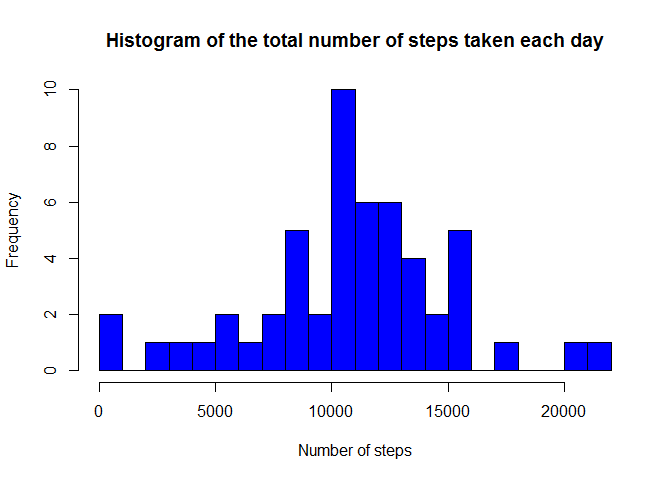
\includegraphics{PA1_template_files/figure-latex/unnamed-chunk-2-1.pdf}

\subsubsection{Calculate and report the mean and median total number of
steps taken per
day}\label{calculate-and-report-the-mean-and-median-total-number-of-steps-taken-per-day}

\begin{Shaded}
\begin{Highlighting}[]
\CommentTok{#mean}
\KeywordTok{mean}\NormalTok{(day_total}\OperatorTok{$}\NormalTok{day_total)}
\end{Highlighting}
\end{Shaded}

\begin{verbatim}
## [1] 10766.19
\end{verbatim}

\begin{Shaded}
\begin{Highlighting}[]
\CommentTok{#median}
\KeywordTok{median}\NormalTok{(day_total}\OperatorTok{$}\NormalTok{day_total)}
\end{Highlighting}
\end{Shaded}

\begin{verbatim}
## [1] 10765
\end{verbatim}

\subsection{What is the average daily activity
pattern?}\label{what-is-the-average-daily-activity-pattern}

\subsubsection{\texorpdfstring{Make a time series plot (type=``l'') of
the 5-minute interval (x-axis) and the average number of steps taken,
averaged across all days
(y-axis)}{Make a time series plot (type=l) of the 5-minute interval (x-axis) and the average number of steps taken, averaged across all days (y-axis)}}\label{make-a-time-series-plot-typel-of-the-5-minute-interval-x-axis-and-the-average-number-of-steps-taken-averaged-across-all-days-y-axis}

\begin{Shaded}
\begin{Highlighting}[]
\NormalTok{day_mean<-}\KeywordTok{with}\NormalTok{(activity_no_NA,}\KeywordTok{tapply}\NormalTok{(steps,interval,mean))}
\NormalTok{day_mean<-}\KeywordTok{as.data.frame}\NormalTok{(day_mean)}
\NormalTok{x<-}\KeywordTok{row.names}\NormalTok{(day_mean)}
\KeywordTok{with}\NormalTok{(day_mean,}\KeywordTok{plot}\NormalTok{(x,day_mean,}\DataTypeTok{type=}\StringTok{"l"}\NormalTok{,}\DataTypeTok{xlab =} \StringTok{"Time interval"}\NormalTok{,}\DataTypeTok{ylab=}\StringTok{"Average number of steps"}\NormalTok{,}\DataTypeTok{main=}\StringTok{"Average daily activity pattern"}\NormalTok{,}\DataTypeTok{col=}\StringTok{"blue"}\NormalTok{))}
\end{Highlighting}
\end{Shaded}

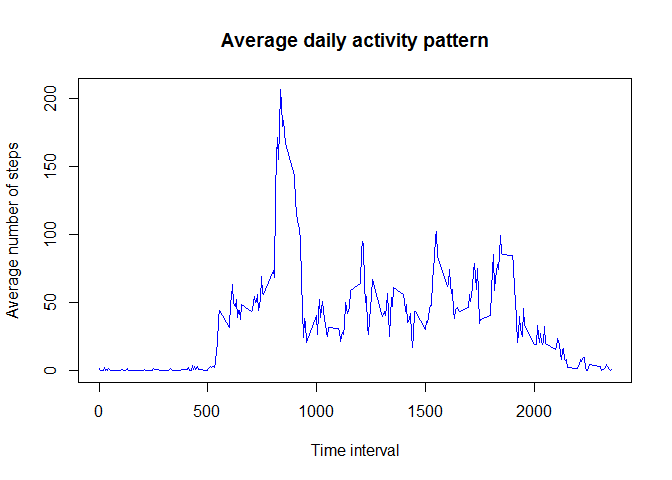
\includegraphics{PA1_template_files/figure-latex/unnamed-chunk-4-1.pdf}

\subsubsection{Which 5-minute interval, on average across all the days
in the dataset, contains the maximum number of
steps?}\label{which-5-minute-interval-on-average-across-all-the-days-in-the-dataset-contains-the-maximum-number-of-steps}

\begin{Shaded}
\begin{Highlighting}[]
\NormalTok{day_mean}\OperatorTok{$}\NormalTok{interval<-x}
\NormalTok{max_interval<-day_mean[}\KeywordTok{which.max}\NormalTok{(day_mean}\OperatorTok{$}\NormalTok{day_mean),]}\OperatorTok{$}\NormalTok{interval}
\NormalTok{max_interval}
\end{Highlighting}
\end{Shaded}

\begin{verbatim}
## [1] "835"
\end{verbatim}

\begin{Shaded}
\begin{Highlighting}[]
\KeywordTok{max}\NormalTok{(day_mean}\OperatorTok{$}\NormalTok{day_mean)}
\end{Highlighting}
\end{Shaded}

\begin{verbatim}
## [1] 206.1698
\end{verbatim}

\subsection{Imputing missing values}\label{imputing-missing-values}

\subsubsection{Calculate and report the total number of missing values
in the dataset (i.e.~the total number of rows with
NAs)}\label{calculate-and-report-the-total-number-of-missing-values-in-the-dataset-i.e.the-total-number-of-rows-with-nas}

\begin{Shaded}
\begin{Highlighting}[]
\CommentTok{#steps variable missing}
\KeywordTok{sum}\NormalTok{(}\KeywordTok{is.na}\NormalTok{(}\KeywordTok{as.character}\NormalTok{(activity}\OperatorTok{$}\NormalTok{steps)))}
\end{Highlighting}
\end{Shaded}

\begin{verbatim}
## [1] 2304
\end{verbatim}

\begin{Shaded}
\begin{Highlighting}[]
\CommentTok{#date variable missing}
\KeywordTok{sum}\NormalTok{(}\KeywordTok{is.na}\NormalTok{(}\KeywordTok{as.character}\NormalTok{(activity}\OperatorTok{$}\NormalTok{date)))}
\end{Highlighting}
\end{Shaded}

\begin{verbatim}
## [1] 0
\end{verbatim}

\begin{Shaded}
\begin{Highlighting}[]
\CommentTok{#interval variable missing}
\KeywordTok{sum}\NormalTok{(}\KeywordTok{is.na}\NormalTok{(}\KeywordTok{as.character}\NormalTok{(activity}\OperatorTok{$}\NormalTok{interval)))}
\end{Highlighting}
\end{Shaded}

\begin{verbatim}
## [1] 0
\end{verbatim}

\subsubsection{Use the mean for the 5-minute interval to impute missing
value and create a new dataset that is equal to the original dataset but
with the missing data filled
in}\label{use-the-mean-for-the-5-minute-interval-to-impute-missing-value-and-create-a-new-dataset-that-is-equal-to-the-original-dataset-but-with-the-missing-data-filled-in}

\begin{Shaded}
\begin{Highlighting}[]
\NormalTok{full_steps<-}\KeywordTok{numeric}\NormalTok{()}
\ControlFlowTok{for}\NormalTok{ (i }\ControlFlowTok{in} \DecValTok{1}\OperatorTok{:}\KeywordTok{length}\NormalTok{(activity}\OperatorTok{$}\NormalTok{steps))\{}
        \ControlFlowTok{if}\NormalTok{(}\KeywordTok{is.na}\NormalTok{(activity}\OperatorTok{$}\NormalTok{steps[i])) \{}
\NormalTok{                steps<-}\KeywordTok{subset}\NormalTok{(day_mean,interval}\OperatorTok{==}\NormalTok{activity}\OperatorTok{$}\NormalTok{interval[i])}\OperatorTok{$}\NormalTok{day_mean}
\NormalTok{        \}}
        \ControlFlowTok{else}\NormalTok{\{}
\NormalTok{                steps<-activity}\OperatorTok{$}\NormalTok{steps[i]}
\NormalTok{        \}}
\NormalTok{        full_steps<-}\KeywordTok{c}\NormalTok{(full_steps,steps)}
\NormalTok{\}  }
\NormalTok{activity_full<-activity}
\NormalTok{activity_full}\OperatorTok{$}\NormalTok{full_steps<-}\StringTok{ }\NormalTok{full_steps   }
\end{Highlighting}
\end{Shaded}

\subsubsection{Make a histogram of the total number of steps taken each
day and Calculate and report the mean and median total number of steps
taken per day. Do these values differ from the estimates from the first
part of the assignment? What is the impact of imputing missing data on
the estimates of the total daily number of
steps?}\label{make-a-histogram-of-the-total-number-of-steps-taken-each-day-and-calculate-and-report-the-mean-and-median-total-number-of-steps-taken-per-day.-do-these-values-differ-from-the-estimates-from-the-first-part-of-the-assignment-what-is-the-impact-of-imputing-missing-data-on-the-estimates-of-the-total-daily-number-of-steps}

\begin{Shaded}
\begin{Highlighting}[]
\NormalTok{day_total_imputed<-}\KeywordTok{with}\NormalTok{(activity_full,}\KeywordTok{tapply}\NormalTok{(full_steps,date,sum))}
\NormalTok{day_total_imputed<-}\KeywordTok{as.data.frame}\NormalTok{(day_total_imputed)}
\KeywordTok{par}\NormalTok{(}\DataTypeTok{mfrow=}\KeywordTok{c}\NormalTok{(}\DecValTok{1}\NormalTok{,}\DecValTok{2}\NormalTok{))}
\KeywordTok{hist}\NormalTok{(day_total_imputed}\OperatorTok{$}\NormalTok{day_total_imputed,}\DataTypeTok{breaks =} \DecValTok{20}\NormalTok{,}\DataTypeTok{col=}\StringTok{"red"}\NormalTok{,}\DataTypeTok{xlab=}\StringTok{"Number of steps"}\NormalTok{,}\DataTypeTok{main=}\StringTok{"Missing value imputed"}\NormalTok{,}\DataTypeTok{ylim=}\KeywordTok{c}\NormalTok{(}\DecValTok{0}\NormalTok{,}\DecValTok{20}\NormalTok{))}
\KeywordTok{hist}\NormalTok{(day_total}\OperatorTok{$}\NormalTok{day_total,}\DataTypeTok{breaks =} \DecValTok{20}\NormalTok{,}\DataTypeTok{col=}\StringTok{"blue"}\NormalTok{,}\DataTypeTok{xlab=}\StringTok{"Number of steps"}\NormalTok{,}\DataTypeTok{main=}\StringTok{"No missing"}\NormalTok{,}\DataTypeTok{ylim=}\KeywordTok{c}\NormalTok{(}\DecValTok{0}\NormalTok{,}\DecValTok{20}\NormalTok{))}
\end{Highlighting}
\end{Shaded}

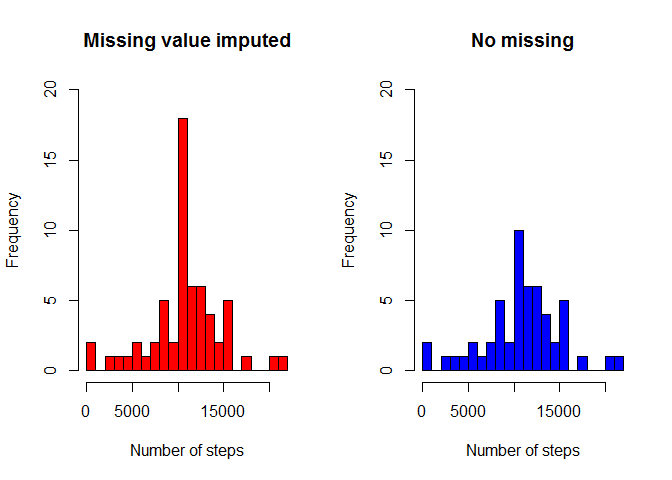
\includegraphics{PA1_template_files/figure-latex/unnamed-chunk-8-1.pdf}

\begin{Shaded}
\begin{Highlighting}[]
\CommentTok{#mean}
\KeywordTok{mean}\NormalTok{(day_total_imputed}\OperatorTok{$}\NormalTok{day_total_imputed)}
\end{Highlighting}
\end{Shaded}

\begin{verbatim}
## [1] 10766.19
\end{verbatim}

\begin{Shaded}
\begin{Highlighting}[]
\CommentTok{#median}
\KeywordTok{median}\NormalTok{(day_total_imputed}\OperatorTok{$}\NormalTok{day_total_imputed)}
\end{Highlighting}
\end{Shaded}

\begin{verbatim}
## [1] 10766.19
\end{verbatim}

\begin{Shaded}
\begin{Highlighting}[]
\CommentTok{#mean difference between imputed and non-imputed results}
\KeywordTok{mean}\NormalTok{(day_total_imputed}\OperatorTok{$}\NormalTok{day_total_imputed)}\OperatorTok{-}\KeywordTok{mean}\NormalTok{(day_total}\OperatorTok{$}\NormalTok{day_total)}
\end{Highlighting}
\end{Shaded}

\begin{verbatim}
## [1] 0
\end{verbatim}

\begin{Shaded}
\begin{Highlighting}[]
\CommentTok{#median difference between imputed and non-imputed results}
\KeywordTok{median}\NormalTok{(day_total_imputed}\OperatorTok{$}\NormalTok{day_total_imputed)}\OperatorTok{-}\KeywordTok{mean}\NormalTok{(day_total}\OperatorTok{$}\NormalTok{day_total)}
\end{Highlighting}
\end{Shaded}

\begin{verbatim}
## [1] 0
\end{verbatim}

So the mean is the same but the median increased

The impact of imputing missing data on the estimates of the total daily
number of steps is on around the total number of steps=10000.

\subsection{Are there differences in activity patterns between weekdays
and
weekends?}\label{are-there-differences-in-activity-patterns-between-weekdays-and-weekends}

\subsubsection{\texorpdfstring{Create a new factor variable in the
dataset with two levels -- ``weekday'' and ``weekend'' indicating
whether a given date is a weekday or weekend
day}{Create a new factor variable in the dataset with two levels -- weekday and weekend indicating whether a given date is a weekday or weekend day}}\label{create-a-new-factor-variable-in-the-dataset-with-two-levels-weekday-and-weekend-indicating-whether-a-given-date-is-a-weekday-or-weekend-day}

\begin{Shaded}
\begin{Highlighting}[]
\NormalTok{activity_full}\OperatorTok{$}\NormalTok{weekdays<-}\KeywordTok{weekdays}\NormalTok{(activity_full}\OperatorTok{$}\NormalTok{date)}
\NormalTok{activity_full}\OperatorTok{$}\NormalTok{is_weekdays<-}\KeywordTok{ifelse}\NormalTok{(}\OperatorTok{!}\NormalTok{(activity_full}\OperatorTok{$}\NormalTok{weekdays }\OperatorTok\StringTok{ }\KeywordTok{c}\NormalTok{(}\StringTok{"Saturday"}\NormalTok{,}\StringTok{"Sunday"}\NormalTok{)),}\StringTok{"Weekdays"}\NormalTok{,}\StringTok{"Weekends"}\NormalTok{)}
\end{Highlighting}
\end{Shaded}

\subsubsection{\texorpdfstring{Make a panel plot containing a time
series plot (i.e.~type = ``l'') of the 5-minute interval (x-axis) and
the average number of steps taken, averaged across all weekday days or
weekend days
(y-axis)}{Make a panel plot containing a time series plot (i.e.~type = l) of the 5-minute interval (x-axis) and the average number of steps taken, averaged across all weekday days or weekend days (y-axis)}}\label{make-a-panel-plot-containing-a-time-series-plot-i.e.type-l-of-the-5-minute-interval-x-axis-and-the-average-number-of-steps-taken-averaged-across-all-weekday-days-or-weekend-days-y-axis}

\begin{Shaded}
\begin{Highlighting}[]
\NormalTok{weekday_mean <-}\StringTok{ }\KeywordTok{aggregate}\NormalTok{(steps }\OperatorTok{~}\StringTok{ }\NormalTok{interval }\OperatorTok{+}\StringTok{ }\NormalTok{is_weekdays, activity_full, mean)}
\KeywordTok{library}\NormalTok{(lattice)}
\KeywordTok{xyplot}\NormalTok{(weekday_mean}\OperatorTok{$}\NormalTok{steps}\OperatorTok{~}\NormalTok{weekday_mean}\OperatorTok{$}\NormalTok{interval}\OperatorTok{|}\NormalTok{weekday_mean}\OperatorTok{$}\NormalTok{is_weekdays,}\DataTypeTok{xlab=}\StringTok{"Interval"}\NormalTok{,}\DataTypeTok{ylab=}\StringTok{"Steps"}\NormalTok{,}\DataTypeTok{layout=}\KeywordTok{c}\NormalTok{(}\DecValTok{1}\NormalTok{,}\DecValTok{2}\NormalTok{),}\DataTypeTok{type=}\StringTok{"l"}\NormalTok{)}
\end{Highlighting}
\end{Shaded}

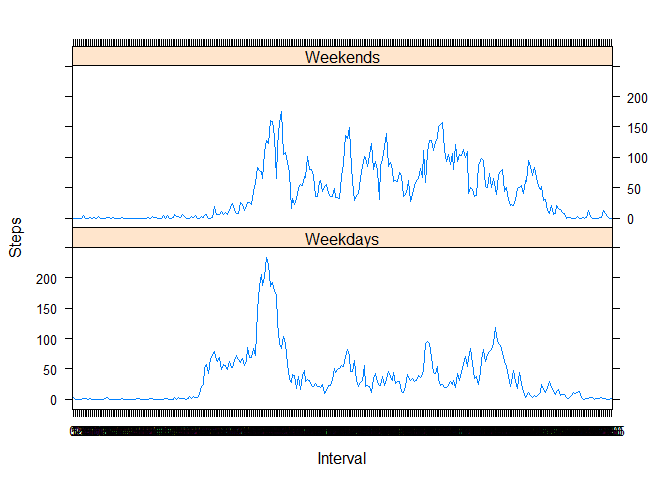
\includegraphics{PA1_template_files/figure-latex/unnamed-chunk-10-1.pdf}


\end{document}
